\subsection{Thực hiện phần cứng}
% Slide 1: Tổng quan phần cứng
\begin{frame}
\frametitle{Thực hiện Phần cứng FDAS}

\begin{block}{Kiến trúc mô-đun}
Hệ thống gồm 2 module hoạt động độc lập:
\begin{itemize}
\item \textbf{Module I}: Thiết bị đeo/Cảm biến - Thu thập chuyển động \& định vị
\item \textbf{Module II}: Camera giám sát - Xác nhận sự kiện qua hình ảnh
\end{itemize}
\end{block}

\begin{columns}
\column{0.5\textwidth}
\begin{alertblock}{Ưu điểm}
\begin{itemize}
\item Linh hoạt triển khai
\item Giám sát phạm vi rộng  
\item Duy trì hoạt động khi 1 module lỗi
\end{itemize}
\end{alertblock}

\column{0.5\textwidth}
\begin{block}{Nguyên lý}
2 nguồn dữ liệu độc lập tăng độ tin cậy phát hiện
\end{block}
\end{columns}

\end{frame}

% Slide 2: Module I - Sơ đồ và sản phẩm thực tế
\begin{frame}
\frametitle{Module I: Thiết bị đeo/Cảm biến}

\begin{columns}
\column{0.5\textwidth}
\begin{figure}[h]
\centering
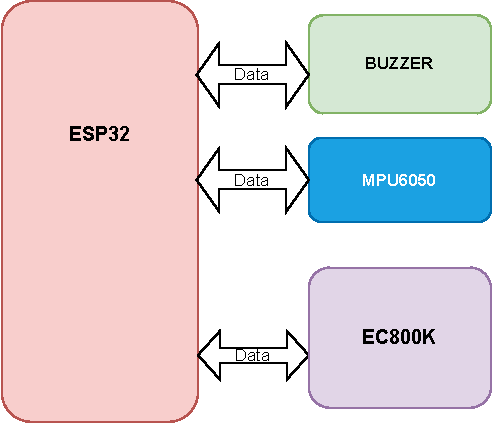
\includegraphics[width=\textwidth]{images/module1_block_diagram-crop.pdf}
\caption{Sơ đồ khối Module I}
\end{figure}

\column{0.5\textwidth}
\begin{figure}[h]
\centering
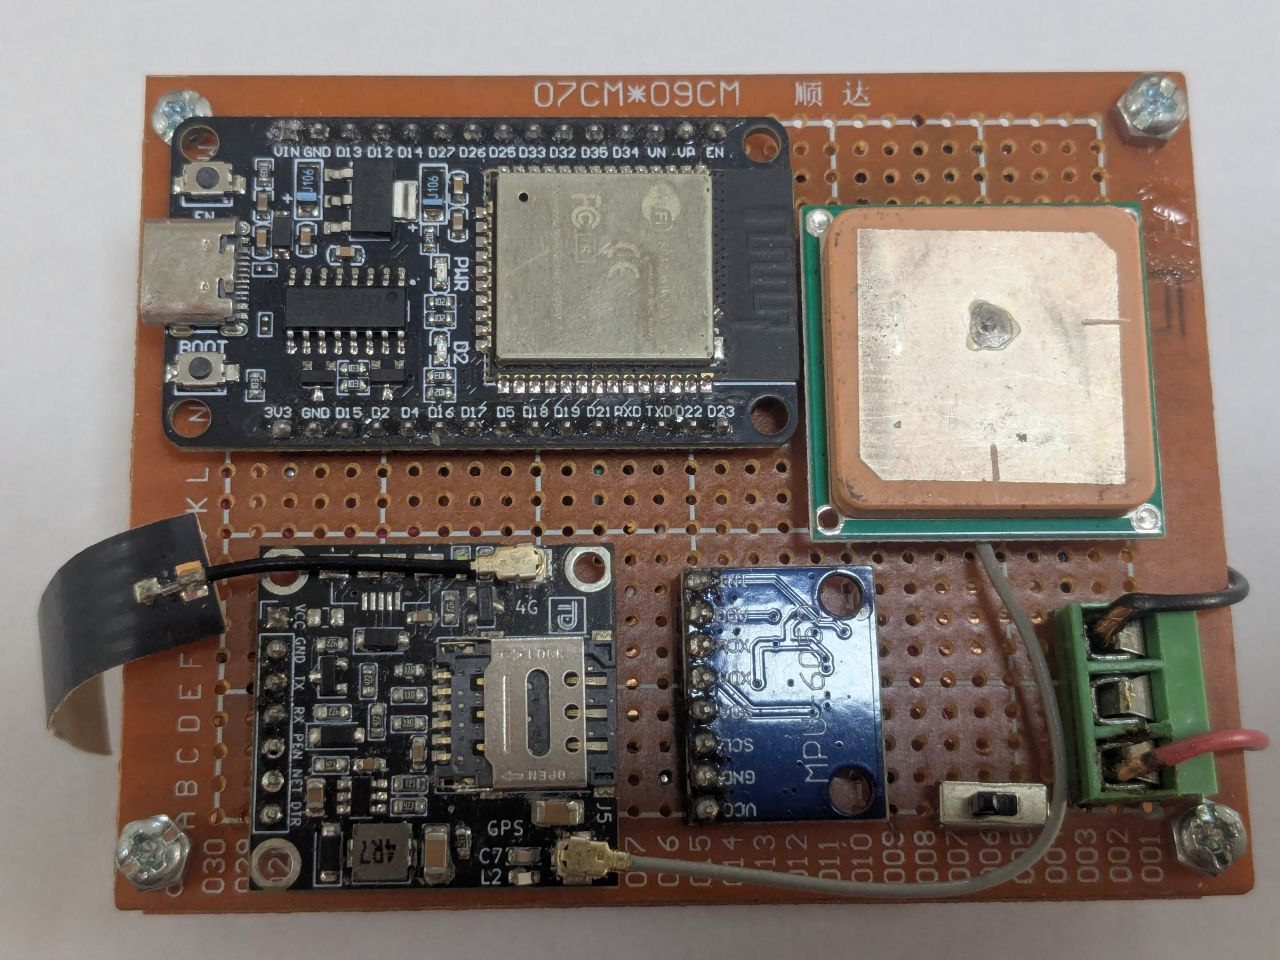
\includegraphics[width=\textwidth]{images/real_board1.jpg}
\caption{Module I thực tế}
\end{figure}
\end{columns}

\begin{block}{Thành phần chính}
\textbf{ESP32-DevKitC-1} (Wi-Fi/BLE) • \textbf{MPU6050} (IMU 6 trục) • \textbf{GPS/4G EC800K} (Định vị) • \textbf{Buzzer/LED} (Cảnh báo)
\end{block}

\end{frame}

% Slide 3: Module II - Camera
\begin{frame}
\frametitle{Module II: Camera giám sát}

\begin{columns}
\column{0.6\textwidth}
\begin{block}{Thành phần chính}
\begin{itemize}
\item \textbf{ESP32-S3-N16R8}:
  \begin{itemize}
  \item Vi điều khiển mạnh mẽ
  \item Tích hợp PSRAM
  \item Giao diện camera chuyên dụng
  \end{itemize}
\item \textbf{Camera OV5640}:
  \begin{itemize}
  \item Cảm biến 5MP
  \item Đa kích thước (QQVGA-UXGA)
  \item Bus 8-bit, 20MHz
  \end{itemize}
\end{itemize}
\end{block}

\column{0.4\textwidth}
\begin{figure}[h]
\centering
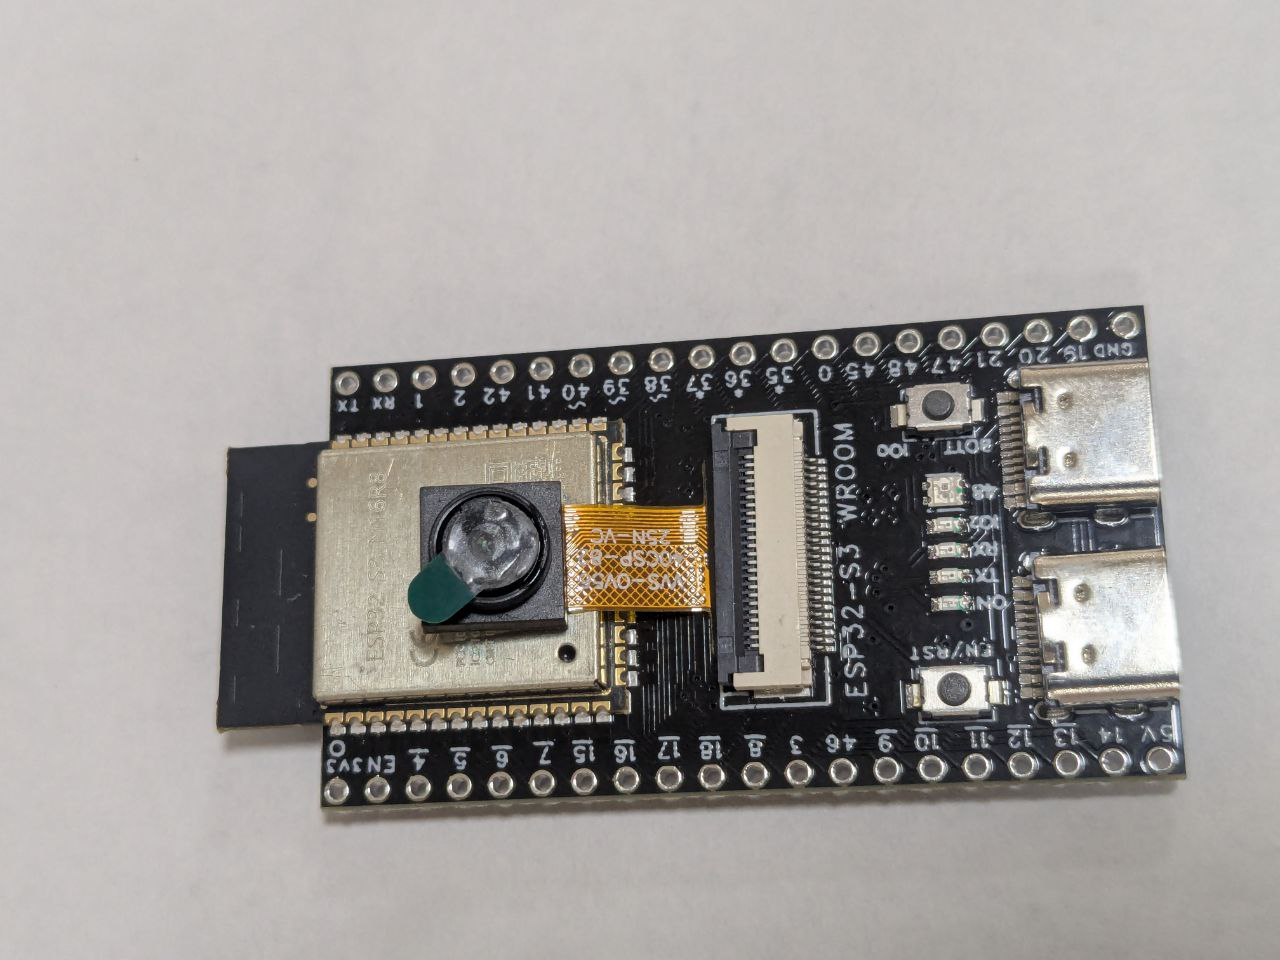
\includegraphics[width=\textwidth]{images/real_board2.jpg}
\caption{Module II thực tế}
\end{figure}
\end{columns}

\end{frame}

% Slide 4: Kết nối phần cứng Module II
\begin{frame}
\frametitle{Kết nối ESP32-S3 ↔ OV5640}

\begin{table}[h]
\centering
\caption{Sơ đồ kết nối chân}
\begin{tabular}{|l|c|l|}
\hline
\textbf{Chức năng} & \textbf{Chân ESP32-S3} & \textbf{Mô tả} \\
\hline
XCLK & 15 & Xung nhịp camera \\
SIOD (SDA) & 4 & Dữ liệu I2C \\
SIOC (SCL) & 5 & Xung nhịp I2C \\
D0-D7 & 11,9,8,10,12,18,17,16 & Bus dữ liệu 8-bit \\
VSYNC & 6 & Đồng bộ dọc \\
HREF & 7 & Tham chiếu ngang \\
PCLK & 13 & Xung nhịp điểm ảnh \\
\hline
\end{tabular}
\end{table}

\begin{alertblock}{Giao tiếp}
SCCB (tương tự I2C) cho cấu hình + Bus song song 8-bit cho dữ liệu
\end{alertblock}

\end{frame}

% Slide 6: Tổng hợp phần cứng - Phần 1
\begin{frame}
\frametitle{Chi phí Phần cứng - Module I}

\begin{table}[h]
\centering
\small
\begin{tabular}{|l|l|r|}
\hline
\textbf{Linh kiện} & \textbf{Chức năng} & \textbf{Giá (VNĐ)} \\
\hline
ESP32-DevKitC-1 & Vi điều khiển chính & 110.000 - 125.000 \\
MPU6050 & Cảm biến IMU 6 trục & 45.000 - 55.000 \\
GPS antenna & Anten nhận GPS & 35.000 - 60.000 \\
GPS/4G EC800K & Định vị \& gửi cảnh báo & ~240.000 \\
Buzzer & Cảnh báo âm thanh & 5.000 - 10.000 \\
\hline
\textbf{Tổng Module I} & & \textbf{~435.000 - 490.000} \\
\hline
\end{tabular}
\end{table}



\end{frame}

% Slide 7: Tổng hợp phần cứng - Phần 2  
\begin{frame}
\frametitle{Chi phí Phần cứng - Module II}

\begin{table}[h]
\centering
\begin{tabular}{|l|l|r|}
\hline
\textbf{Linh kiện} & \textbf{Chức năng} & \textbf{Giá (VNĐ)} \\
\hline
ESP32-S3-N16R8 & Vi điều khiển xử lý ảnh & 275.000 - 300.000 \\
Camera OV5640 & Cảm biến hình ảnh 5MP & 150.000 - 200.000 \\
\hline
\textbf{Tổng Module II} & & \textbf{~425.000 - 500.000} \\
\hline
\hline
\textbf{TỔNG HỆ THỐNG} & & \textbf{~860.000 - 990.000} \\
\hline
\end{tabular}
\end{table}


\end{frame}
